\section{Networks}
\label{sec:methodology}
%\hbadness=99999

Given a query $q = (c_1^q, \ldots, c_i^q, \ldots, c_n^q)$, our model predicts label sequence $\bm{y} = (y_1, \ldots, y_i, \ldots, y_n)$ where $y_i$ is the label of character $c_i^q$. BiLSTM-CRF is a typical deep learning model to deal with sequence labelling task. BiLSTM-CRF can be used for query segmentation task directly. The input to BiLSTM-CRF is a the sequence of characters in $q$. Then a BiLSTM module encodes this character sequence, and get a feature sequence. The final CRF module will decode the label sequence $\bm{y}$ based on the feature sequence. In such common BiLSTM-CRF model, label $y_i$ of $c_i^q$ only relies on the characters in $q$. Now, for each character $c_i^q$ we extract a feature bag $F_i$ from external documents which can provide helpful boundary information. To take advantage of $F_i$, we extend the common BiLSTM-CRF model by adding an additional module which take $F_i$ as anothe input. The feature bag $F_i$ is extract from several contexts. We argue that the boundary information carried by different contexts is not equally importance. Therefore this added module uses attention mechanism to make this difference.

Figure \ref{fig:12} shows the architecture of our model. This architecture consists of $3$ modules, a query encoder, a feature encoder and a label decoder. Query encoder and label decoder are responsible for encoding the character sequence of a query and decoding the label sequence respectively. These two modules are from the common BiLSTM-CRF model. The feature encoder is our designed attention based module which encodes the feature bag.

\begin{figure*}
	\centering
	\begin{subfigure}[b]{1\columnwidth}
		\centering
		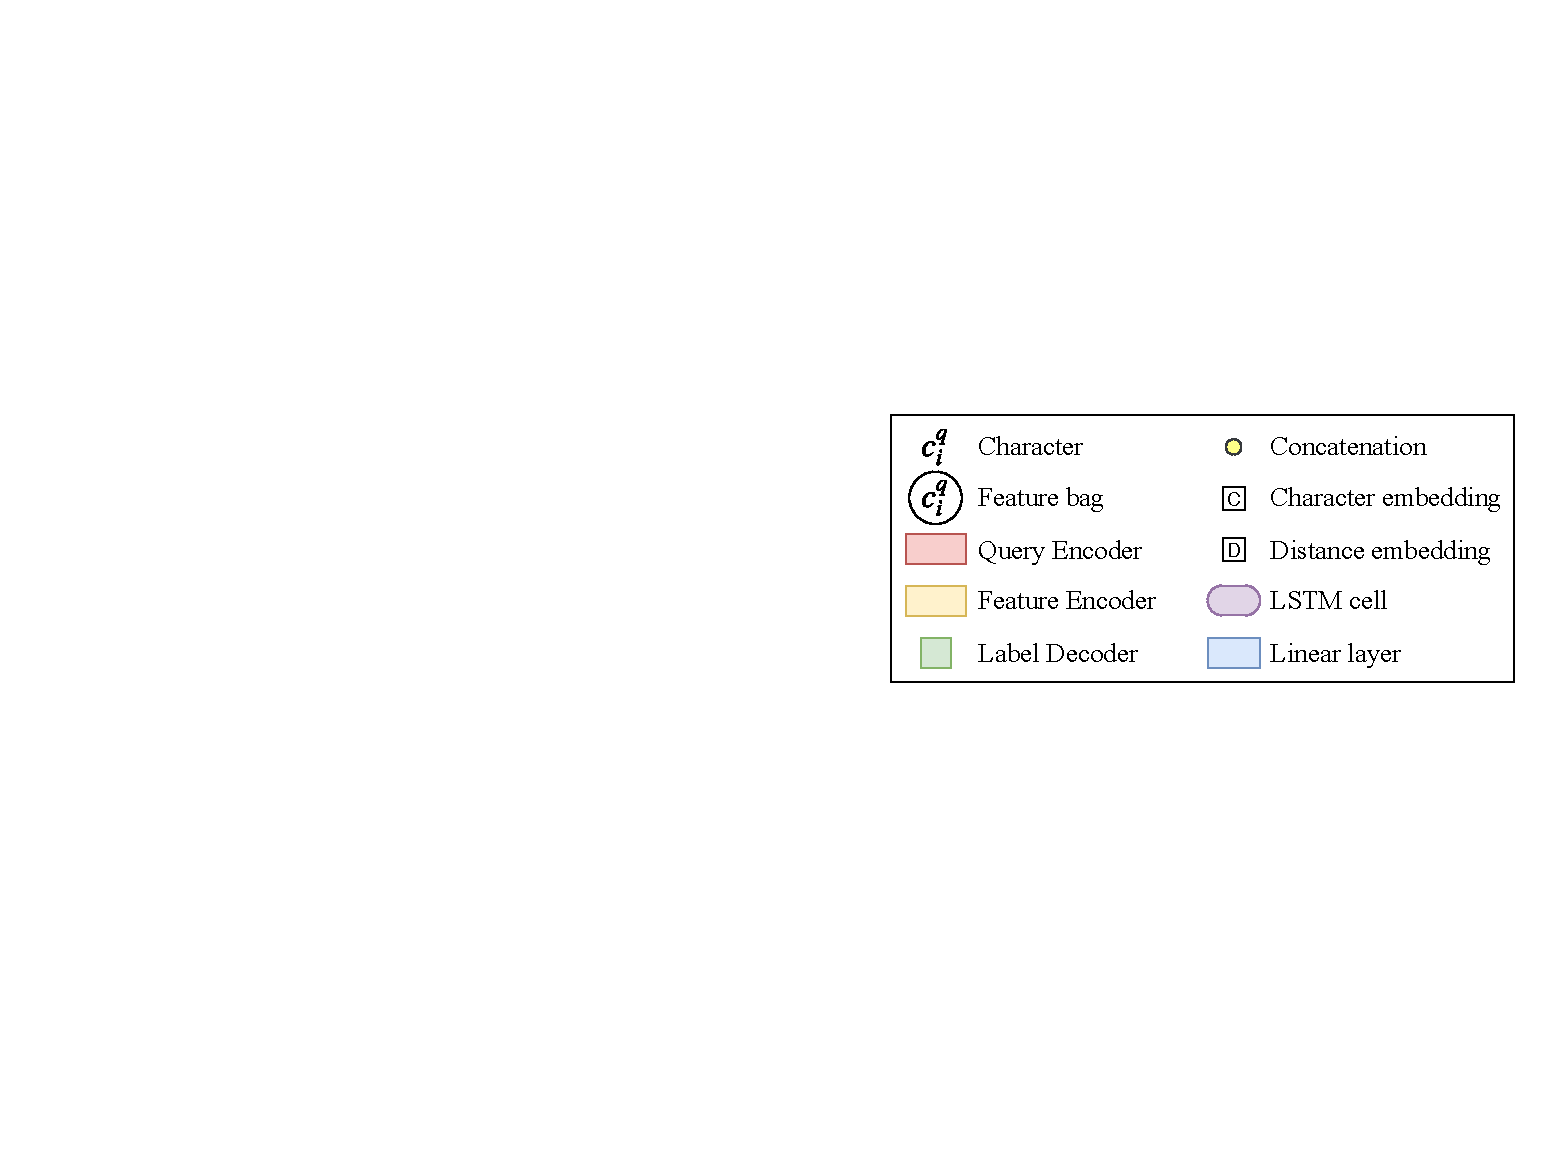
\includegraphics[width=0.85\columnwidth]{figures/model-1.pdf}
		\caption[]%
		{{\small Legend.}}
		\label{fig:11}
	\end{subfigure}
	\hfill
	\begin{subfigure}[b]{1\columnwidth}
		\centering
		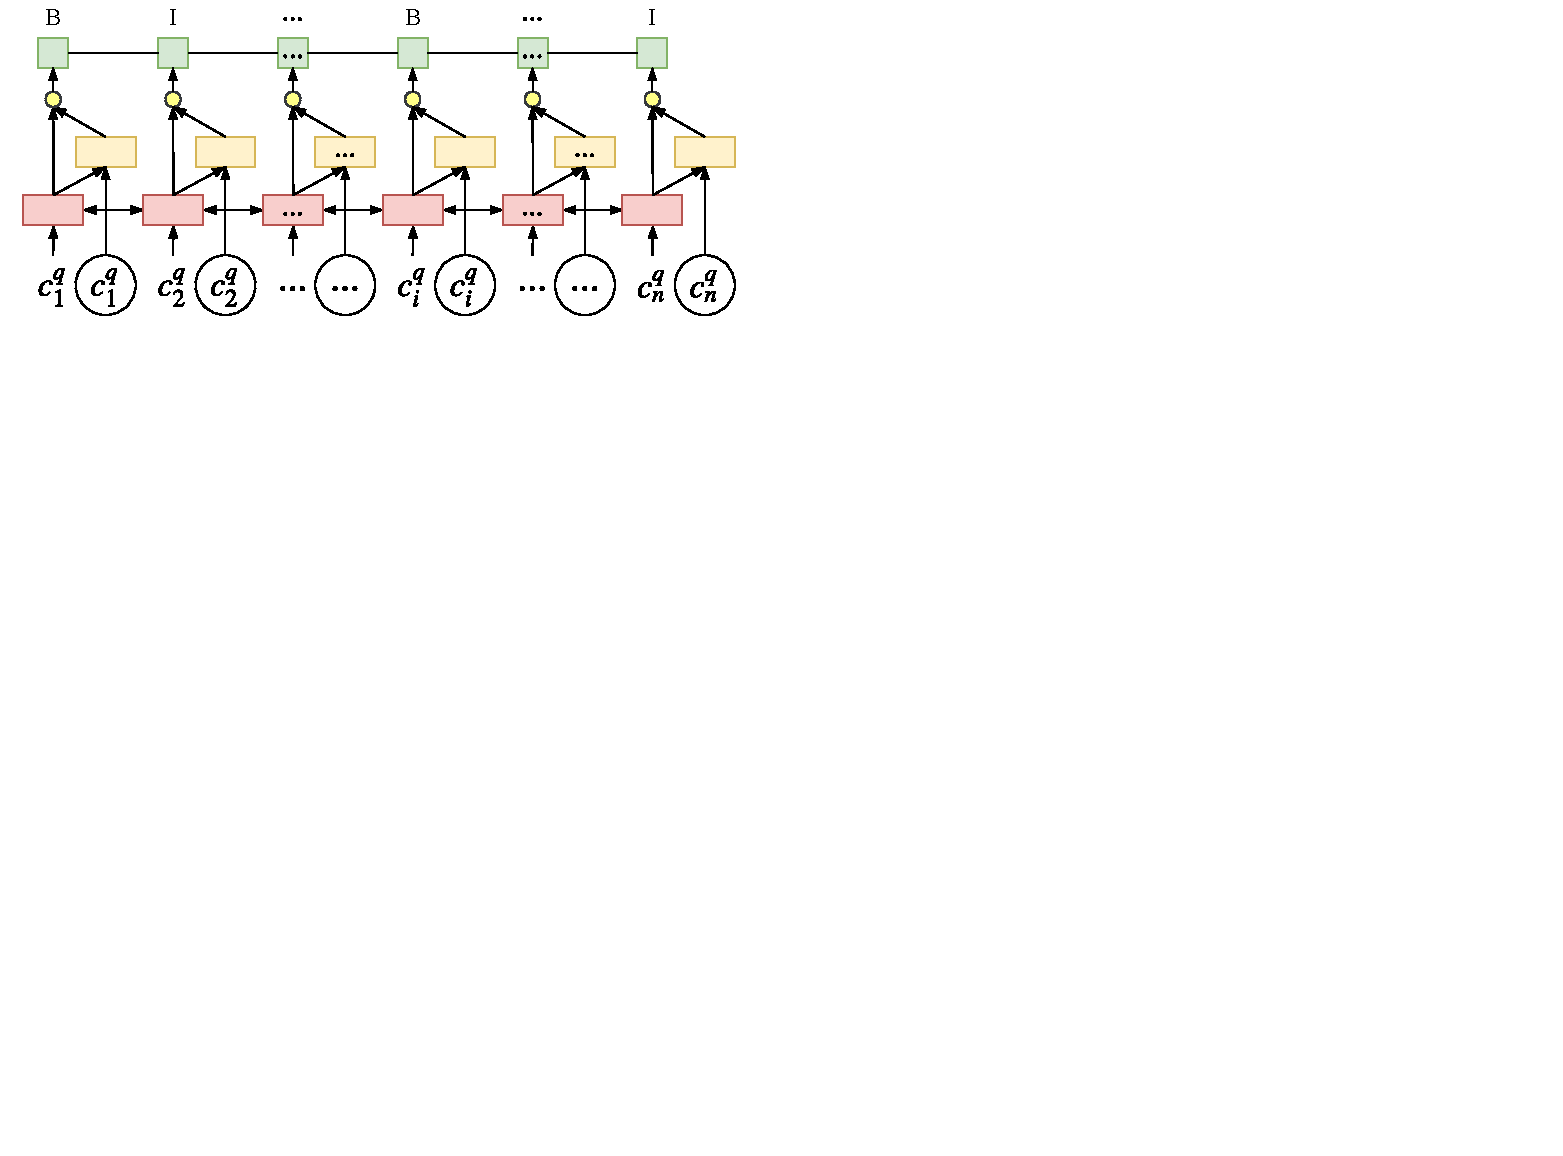
\includegraphics[width=0.9\columnwidth]{figures/model-2.pdf}
		\caption[]%
		{{\small Architecture.}}
		\label{fig:12}
	\end{subfigure}
	\vskip
	\baselineskip
	\begin{subfigure}[b]{1\columnwidth}
		\centering
		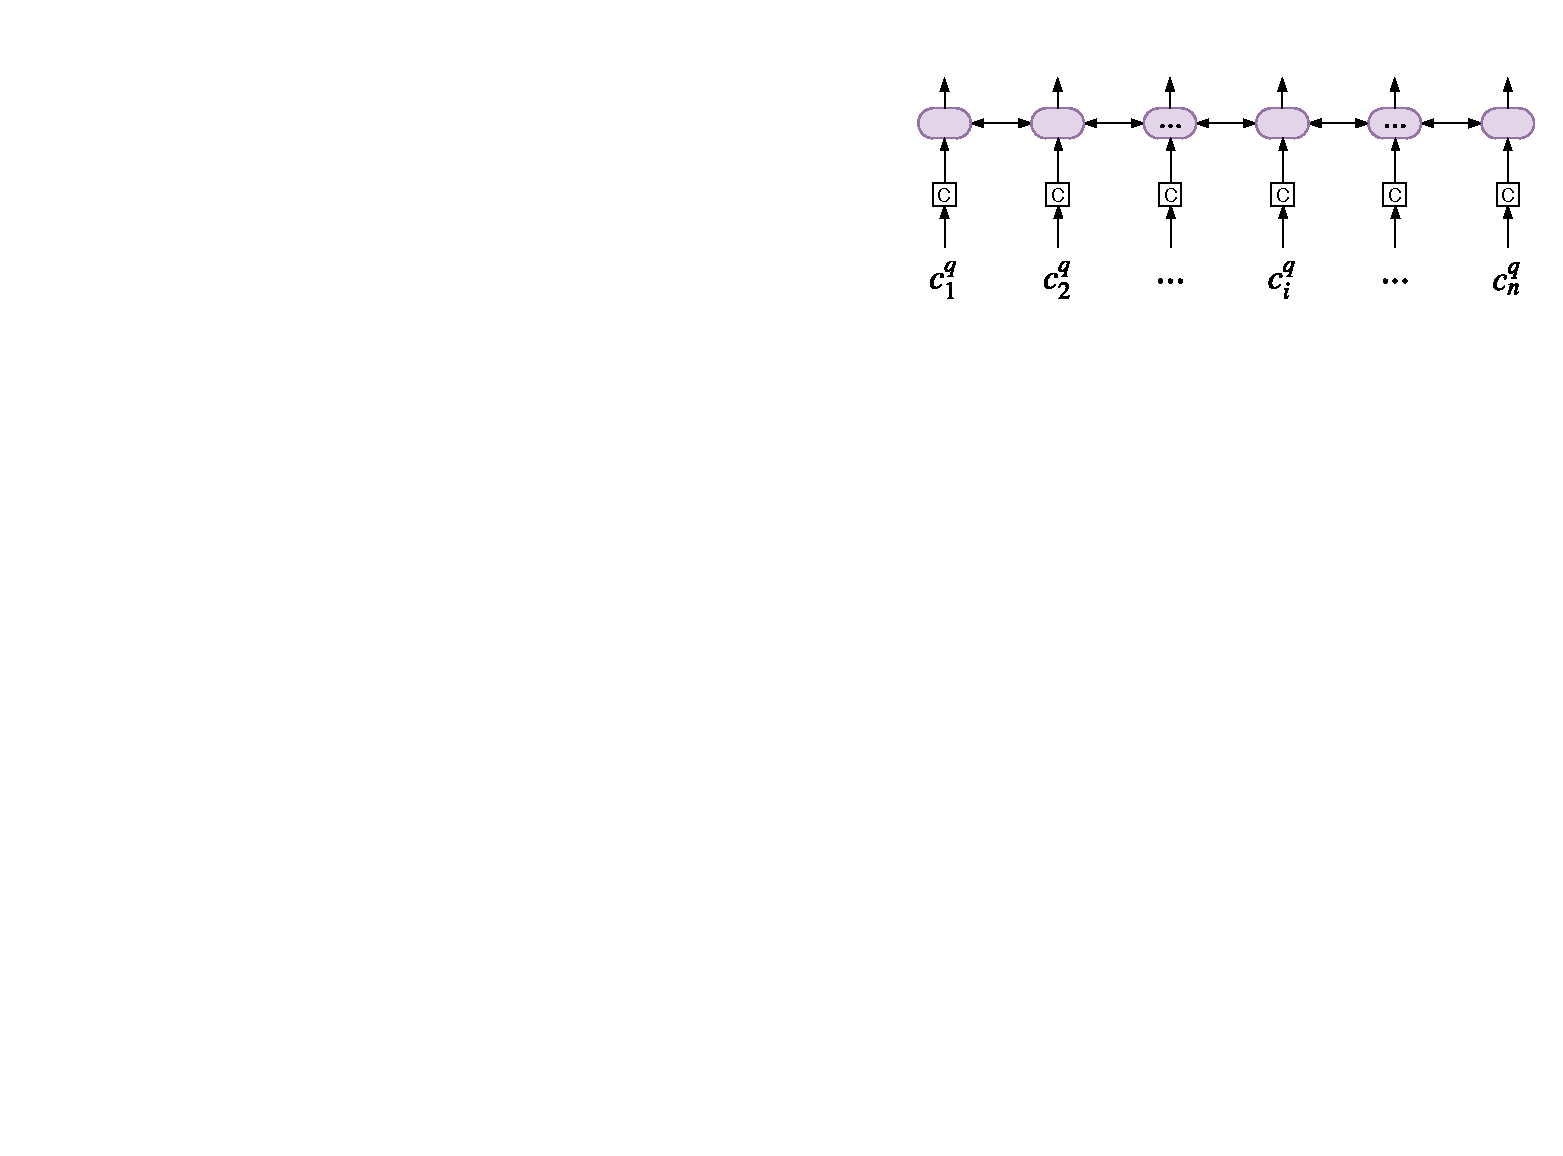
\includegraphics[width=0.9\columnwidth]{figures/model-3.pdf}
		\caption[]%
		{{\small Query Encoder.}}
		\label{fig:21}
	\end{subfigure}
	% \quad
	\hfill
	\begin{subfigure}[b]{1\columnwidth}
		\centering
		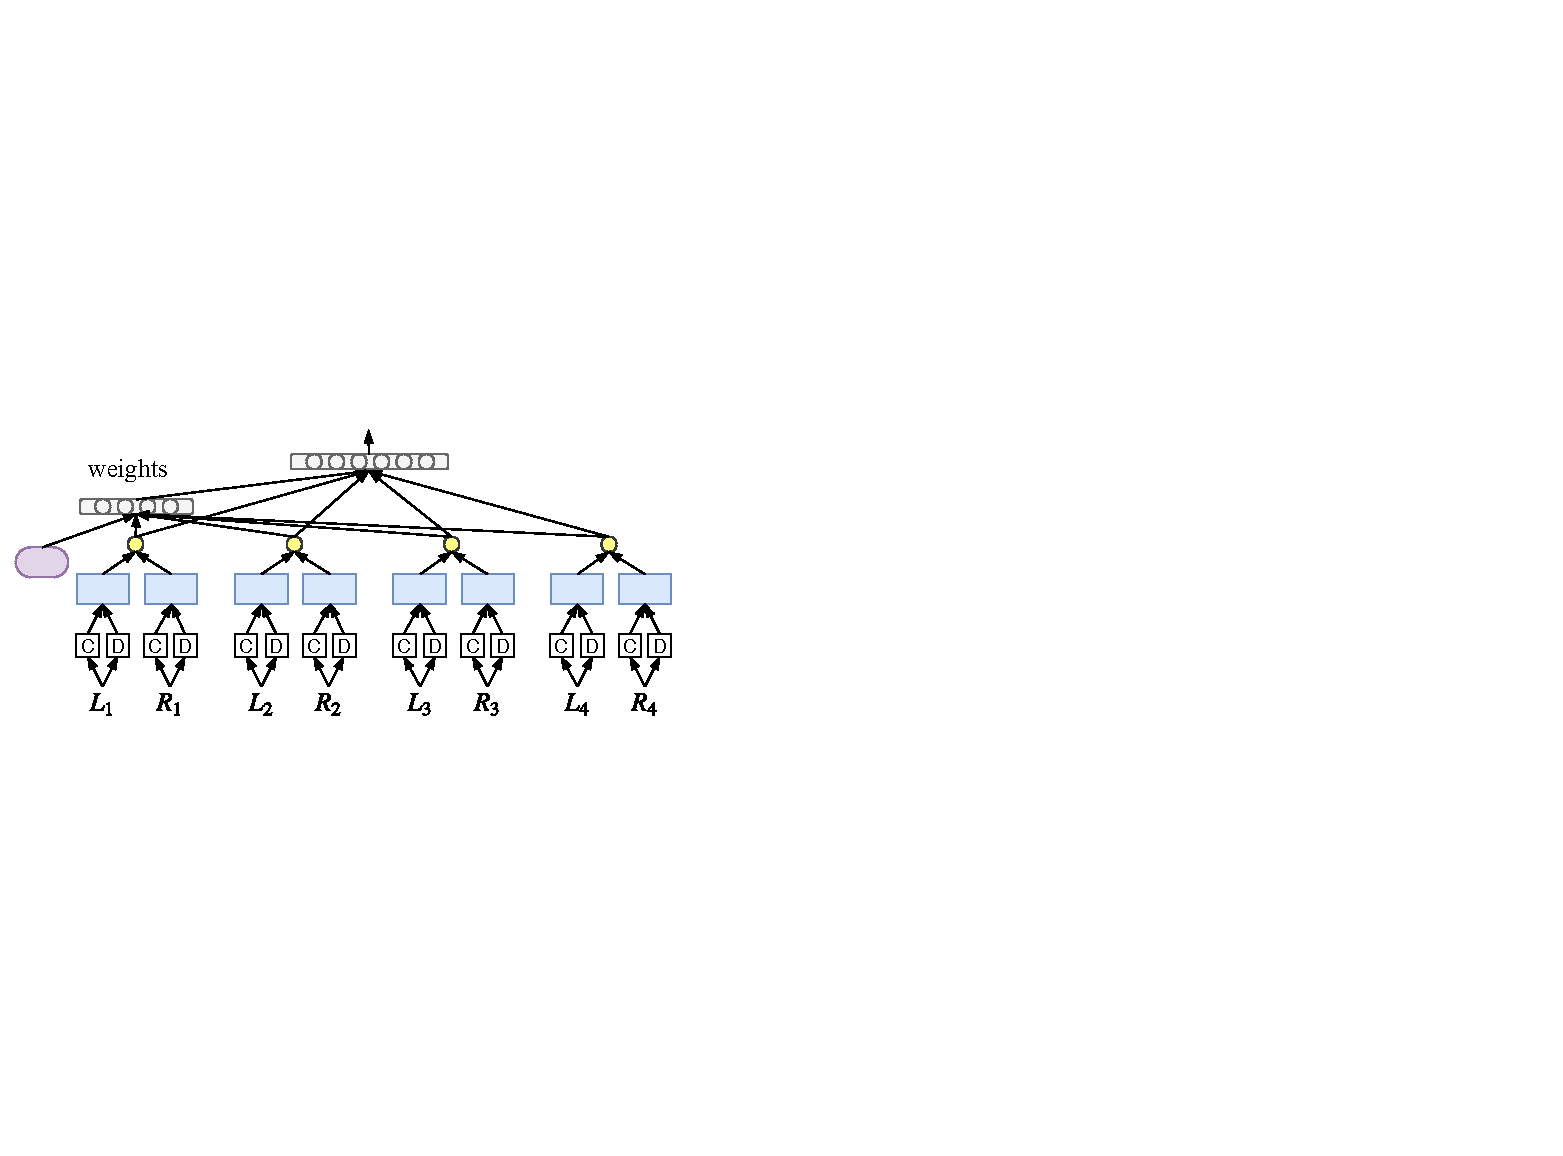
\includegraphics[width=0.9\columnwidth]{figures/model-4.pdf}
		\caption[]%
		{{\small Feature Encoder.}}
		\label{fig:22}
	\end{subfigure}
	\caption[]
	{\small There are 4 sub-figures, Legend, Architecture, Query Encoder and Feature Encoder. (a) shows all legends used in other 3 subfigures. (b) is the architecture of our model which contains three module, Query Encoder, Feature Encoder and Label Decoder. (c) shows the detail of query encoder module which is a LSTM structure. (d) shows the detail of feature encoder module which is based on the attention mechanism.}
	\label{fig:model}
	\vspace{-10pt}
\end{figure*}

\subsection{Query Encoder}

As shown in Figure \ref{fig:21}, the query encoder is a BiLSTM structure. The BiLSTM structure consists of two reverse direction LSTM, forward and backward.

Assuming the set of all used Chinese characters is $\mathcal{C}$ and its size is $|\mathcal{C}|$, each character $c_i^q$ in query $q$ can be represented as a 1-Hot vector $H(c_i^q)$ with length $|\mathcal{C}|$. We initialize the character embedding $E_c$ with standard normal distribution. The hidden states of character $c_i^q$ are as follows.
\begin{align*}
	\overrightarrow{h_i} & = LSTM(\overrightarrow{h_{i-1}}, H(c_i^q) E_c),
	\\
	\overleftarrow{h_i}  & = LSTM(\overleftarrow{h_{i+1}}, H(c_i^q) E_c),
\end{align*}
$\overrightarrow{h_i}$ is the forward hidden state, while $\overleftarrow{h_i}$ is the backward hidden state. The concatenation $h_i=[\overrightarrow{h_i}; \overleftarrow{h_i}]$ of $\overrightarrow{h_i}$ and $\overleftarrow{h_i}$ is treated as the full hidden state of character $c_i^q$.



\subsection{Feature Encoder}

As for each character $c_i^q$ in query $q$, its feature bag is $F_i$, and $\left \langle L, R \right \rangle \in F_i$ is the features from one context. In feature encoder, because $L$ and $R$ contains same kinds of features, same network structure can be used to encode them. Fig \ref{fig:22} shows the structure of feature encoder.

% The representation vectors of $L_j$ and $R_j$ are concatenated. This concatenated vector $f_j$ is treated as the representation of all boundary information from the $j$th context. Then the attention is applied on $(f_1, f_2, \cdots, f_j, \cdots)$ according to the hidden state $h_i$ of $c_i^q$. 

Assuming the window size is $w$, both $L$ and $R$ contain $w$ characters and a distant number $k$. We can use the following structure to accept both left and right features:
\begin{align*}
	e^c = \frac{1} {w} \sum_{c} {H(c)E_c}, \ \ e^d = G(k)E_d.
\end{align*}
$H(c)$ is the 1-Hot vector of character $c$. $E_c$ is the same character embedding which has been used in Query Encoder. We just average the embedding of characters in $\mathcal{C}$ as the representation of character features. $G(k)$ is the 1-Hot vector of distant number $k$ whose dimension depends on the range that $k$ can take. The max value of $k$ is not larger than the max length of all segments. $E_d$ is the distance embedding matrix which is initialized by standard normal distribution.

We concatenate character feature vector $e^c$ and distance feature vector $e^d$ as the whole representation of $L$ or $R$. Then a linear layer is applied on $e$ to integrate character and distance features.
\begin{align*}
	e = [e^c; e^d], \ \ g = \tanh(We).
\end{align*}

By applying above operations to $\left \langle L_j, R_j \right \rangle \in F_i$, we can get the $g_l$ for left features $L_j$ and $g_r$ for right features $R_j$. The concatenation $f_i = [g_l; g_r]$ is treat as the full representation of the $j$th context.

$(f_1, f_2, \ldots, f_j, \ldots)$ are feature vectors of all context in feature bag $F_i$. We use the following formulas to calculate the weights $(\alpha_1, \alpha_2, \ldots, \alpha_j, \ldots)$ where $\alpha_i$ is the weight of $f_i$.
\begin{align*}
	w_j = \tanh(f_j^TU)h_i, \ \ \alpha_j = \frac{\exp{(w_j)}}{\sum_t \exp{(w_t)}},
\end{align*}
where $h_i$ is the hidden state of BiLSTM of the character $c_i^q$ from the query encoder. Because $h_i$ is strongly related to the label of character $c_i^q$. The context feature $f_j$ which is more related to $h_i$ should receive more attention. $U$ is a matrix with size $|f_j| \times |h_i|$.  Finally, the context bag representation $b_i$ are the weighted sum of each $f_j$.
\begin{align*}
	b_i = \sum_j^M \alpha_j f_j.
\end{align*}


\subsection{Label Decoder}
Label decoder module uses a CRF layer to predict the label sequence $\bm{y} = (y_1,  \ldots, y_i, \ldots, y_n)$, where $y_i$ is the label of $c_i^q$. CRF has been used widely in many sequence labeling tasks. Assuming the input to CRF layer is $\bm{z} = (z_1, \ldots, z_i, \ldots, z_n)$, where $z_i$ can be treat as full vector representation of character $c_i^q$. The conditional probability of any possible label sequence $\bm{y}$ given $\bm{z}$ of query $q$ can be formalized as follow,
\begin{align*}
	p(\bm{y} | \bm{z}) & = \frac{\prod_{i=1}^n \phi(y_{i-1}, y_i, z_i)} {\sum_{y' \in \mathcal{Y}(z)}\prod_{i=1}^n \phi(y_{i-1}', y_i', z_i)}, \\
	\phi(y', y, z)     & = \exp(W_{y', y}^T z).
\end{align*}
Where $\phi(*)$ is potential function. $W_{y', y}$ is the weight vector corresponding to label pair $(y', y)$. Parameters can be learnt by maximizing the log-likelihood,
\begin{align*}
	L(W) = \sum_{z \ of \ q \in Q} \log p(y|z).
\end{align*}

There are 3 methods to choose vector $z_i$ for character $c_i^q$. First method is $z_i = h_i$. Only the hidden state of characters in $q$ are used to predict labels, which is the common BiLSTM-CRF model. Because this method only take the query itself into consideration, we call it BiLSTM-CRF(Q). Second method is $z_i = b_i$, which predicts labels mainly based on contexts. This method is called BiLSTM-CRF(C). In last method, $z_i = [h_i; b_i]$ concatenates the hidden state $h_i$ and context bag information $b_i$. This method called BiLSTM-CRF(Q+C) relies on both the query and contexts.

